\documentclass[convert={density=100,outext=.png}]{standalone}
\usepackage{tikz}


\begin{document}
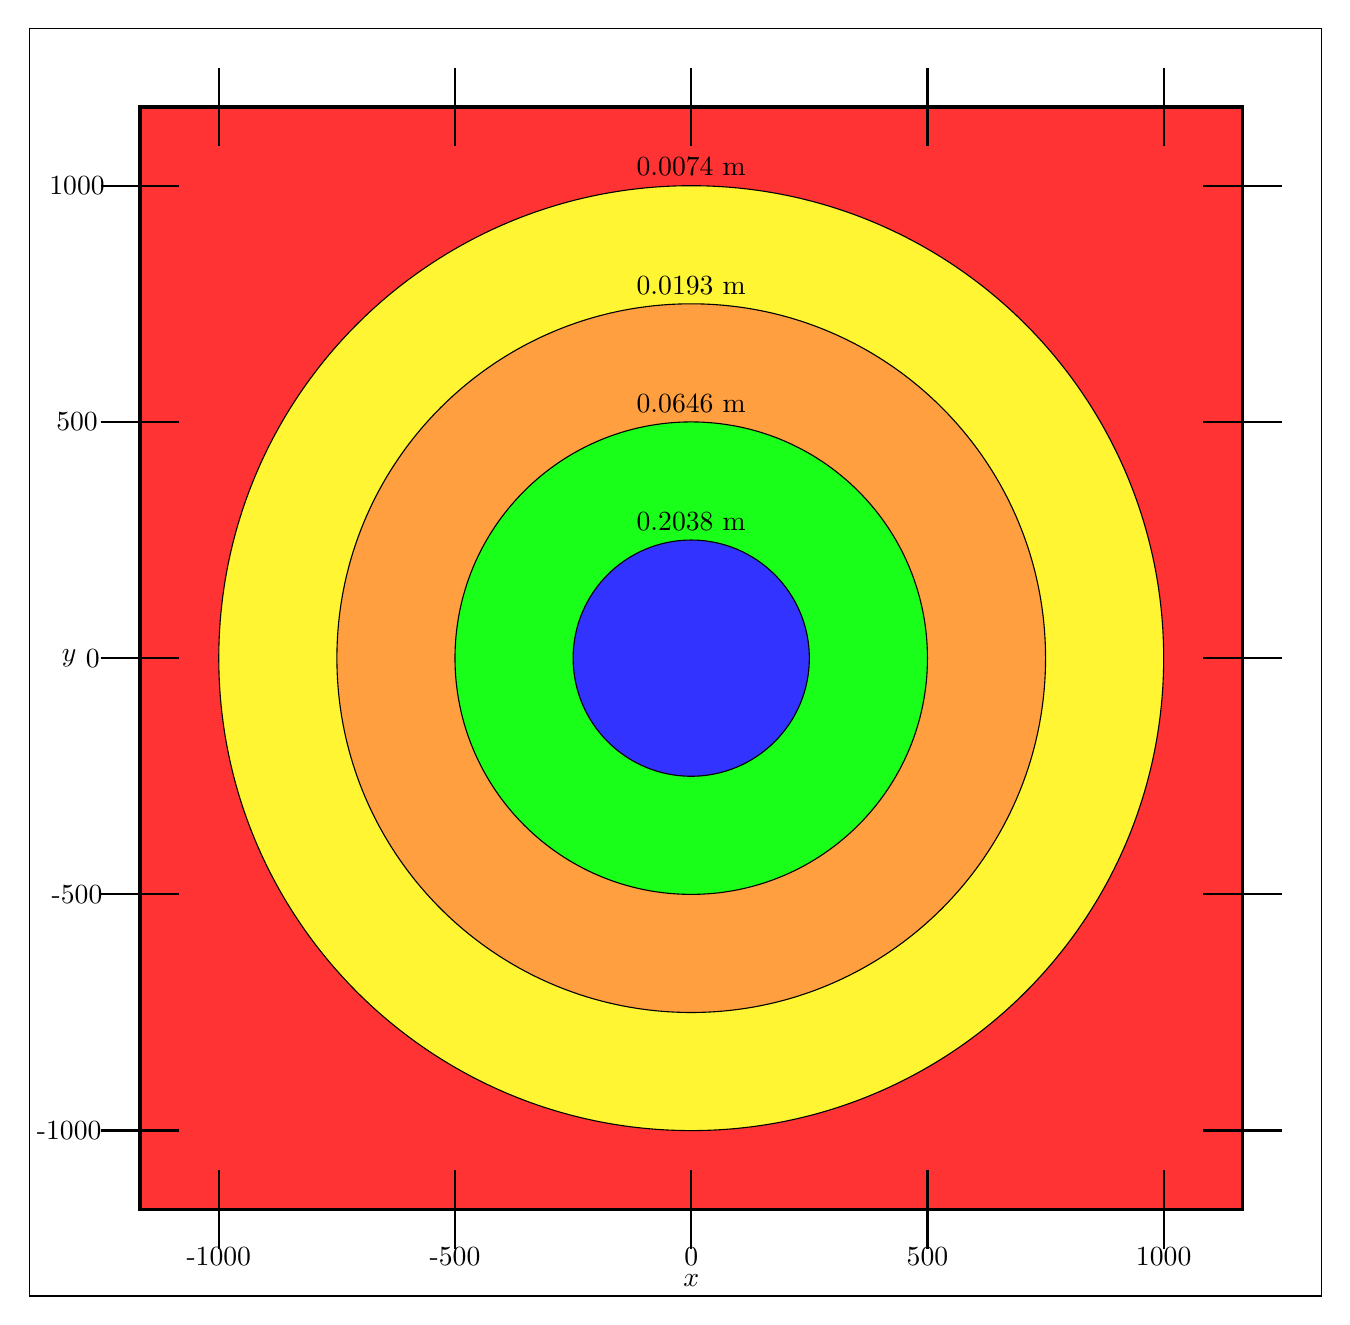
\begin{tikzpicture}

%draws the background sqaure and color coordinated cicles
\draw[fill=white] (-8.4,-8.1) rectangle (8,8);
\draw[fill=red!80,very thick] (-7,-7) rectangle (7,7);
\draw[fill=yellow!80] (0,0) circle (6);
\draw[fill=orange!75] (0,0) circle(4.5);
\draw[fill=green!90] (0,0) circle(3);
\draw[fill=blue!80] (0,0) circle(1.5);

%draws grid
\foreach \x in {-6,-3,...,6}
    \draw[thick] (\x,-7.5) -- (\x,-6.5)  (\x,7.5) -- (\x,6.5);
\foreach \y in {-6,-3,...,6}
    \draw[thick] (-7.5,\y) -- (-6.5,\y) (7.5,\y) -- (6.5,\y);

%label grid
\draw (-6,-7.6) node {-1000};
\draw (-3,-7.6) node {-500};
\draw (0,-7.6) node {0};
\draw (0,-7.9) node {$x$};
\draw (3,-7.6) node {500};
\draw (6,-7.6) node {1000};

\draw (-7.9,-6) node {-1000};
\draw (-7.8,-3) node {-500};
\draw (-7.6,0) node {0};
\draw (-7.9,0) node {$y$};
\draw (-7.8, 3) node {500};
\draw (-7.8, 6) node {1000};

\draw (0,1.5) node[anchor=south] {0.2038 m};
\draw (0,3) node[anchor=south] {0.0646 m};
\draw (0,4.5) node[anchor=south] {0.0193 m};
\draw (0,6) node[anchor=south] {0.0074 m };



\end{tikzpicture}
\end{document}
